% Titre : ADN - liste
% Filiere : BCPST
% Difficulte :
% Type : DS, DM
% Categories : info
% Subcategories : 
% Keywords : info



\begin{exercice}[Informatique]
Les questions sont plus ou moins indépendantes. Toutes les fonctions écrites (ou mentionnées) dans les questions précédentes peuvent être utilisées a posteriori. \\


Il est devenu habituel de dire que l'ADN se présente comme un texte composé à l'aide de quatre lettres A,C,G,T, qui s'enchaînent sans interruption et qui est orienté avec un début et une fin. 

%On suppose que l'on a à notre disposition une chaine de caractères, appelée \texttt{ADN}, dont les caractères sont les lettres 'A','C','G' ou 'T'. 

On souhaite faire une étude statistique des lettres présentes dans une séquence d'ADN. 
\begin{enumerate}
\item \begin{enumerate}


\item Ecrire une fonction \texttt{frequence\_A} qui prend en argument une chaine de caractères \texttt{ADN}  et qui retourne la fréquence de la lettre A dans cette chaîne. 

\item On souhaite comparer la fréquence d'apparition de la lettre 'A' entre deux séquences d'ADN. Ecrire une fonction Python \texttt{compare} qui prend en argument deux chaines de caractères \texttt{ADN1}, \texttt{ADN2} et retourne 'elles sont proches' si la fréquence de la lettre A dans \texttt{ADN1} et dans \texttt{ADN2} différe de moins de 0.01. La fonction retournera 'elles ne sont pas proches' dans le cas contraire. \\
\end{enumerate}

On s'intéresse maintenant aux acides aminés, il faut alors regarder les codons qui se lisent par trois (cf le tableau de la dernière page), on doit donc diviser la chaîne de caractères par codon. 

\item
\begin{enumerate}
\item Completer (sur votre copie) la fonction \texttt{liste\_codon}  python qui prend en argument une chaine de caractère \texttt{ADN} et qui  retourne une liste dont les éléments sont les codons de la chaîne. (On supposera que la longueur de la chaine de caractères est bien divisible par 3 sans le vérifier dans la fonction) 
\begin{lstlisting}
def liste_codon(ADN):
    L=[]
    for i in range(0,  ,  ):
        L=L+[ADN[  :  ]]
    return(L)
\end{lstlisting}

Exemple : si \texttt{ADN='GCAGAGTTTTGGTGC'}, la liste retournée sera :
\texttt{['GCA','GAG', 'TTT','TGG','TGC']}.\\
 
 \item On suppose que l'on a  créé une liste \texttt{code\_genetique} qui contient tous les codons possibles. \texttt{code\_genetique=['GCA','GCC', 'GCG', ...., 'TAG', 'TGA']}\\
 
Quelle est la longueur de la liste \texttt{code\_genetique} ? Comment obtenir cette longueur avec une commande Python ? \\

\item On suppose que l'on a une chaine de caractères \texttt{ADN} à notre disposition. 
Ecrire une fonction python \texttt{test} qui vérifie si chaque codons de la liste \texttt{L=liste\_codon(ADN)} est bien un codon du code génétique. \\

\item Compléter (sur votre copie) la fonction \texttt{start} qui prend en argument une liste de codons et qui retourne  l'indice de la première fois où l'on trouve le codon START ('ATG'). Si jamais il n'y en a pas, elle devra retourner un message d'erreur. \\ 
\begin{lstlisting}
def start(L):
    i=0
    while L[i]          :
        if i<len(L)-1:
            
        else:
            return('pas de codon START')
    return(  )
\end{lstlisting}

(Vous pouvez aussi proposer une fonction différente si vous ne comprenez pas la logique de celle-ci, mais attention aux problèmes d'indices.) 

\item Ecrire une fonction \texttt{stop} qui prend en argument une liste de codons et qui retourne  l'indice de la première fois où l'on trouve un codon STOP. Si jamais il n'y en a pas, elle devra retourner un message d'erreur. \\

\item Ecrire une fonction \texttt{proteine} qui prend en argument une liste de codons et  retourne la sous-liste des codons entre   le premier codon START et le premier codon STOP après ce codon START.  (Cette sous-liste contiendra les deux codons START et STOP. On ne  se penchera pas sur le problème d'erreurs, et on supposera que  notre liste contient bien un codon START et un codon STOP dans le bon ordre)   \\
\end{enumerate}






A une séquence d’ADN  correspond une unique séquence d’ARN grâce aux règles de complémentarité : G  et   C sont inversé, A devient U et T devient A. Par exemple, la séquence d’ADN 'AATCGA' est transcrite en 'UUAGCU.' 
\item 
\begin{enumerate}

\item Compléter (sur votre copie)  la fonction python  \texttt{transcription\_lettre} qui prend en argument une lettre correspondant à de l'ADN et qui retourne la lettre d'ARN correspondante. 
\begin{lstlisting}
def transcription_lettre(lettre):
	if lettre==   :
		lettre='G'
	elif          :
		lettre='C'
	elif lettre=='A':
	
	elif          :
		lettre=
    return(       )
\end{lstlisting}

\item Ecrire une fonction python \texttt{transcription} qui prend en argument une chaine de caractères correspondant à de l'ADN et qui retourne la chaine de caractères d'ARN correspondante. 


Parfois il y  a  des erreurs dans la transcription et une lettre est mal transmise. 

\item Ecrire une fonction python \texttt{mutation} qui prend en argument une chaine de caractères (correspondant à de l'ADN) et qui retourne une  chaine de caractères où les lettres 'C' et 'G' sont inversées avec probabilité  99\% et non inversée avec probabilité 1\%, la lettre 'A' est bien changée en 'U' avec probabilité 99\% et changée en 'C' avec probabilité 1\% et la lettre 'T' devient la  lettre 'A' avec proba 99\% et changée en 'U' avec proba 1\%  . Après l'avoir importée, on pourra utiliser la fonction random() qui retourne un réel aléatoire entre 0 et 1. 

\end{enumerate}

\end{enumerate}


\end{exercice}



\begin{figure}[h]
\centering
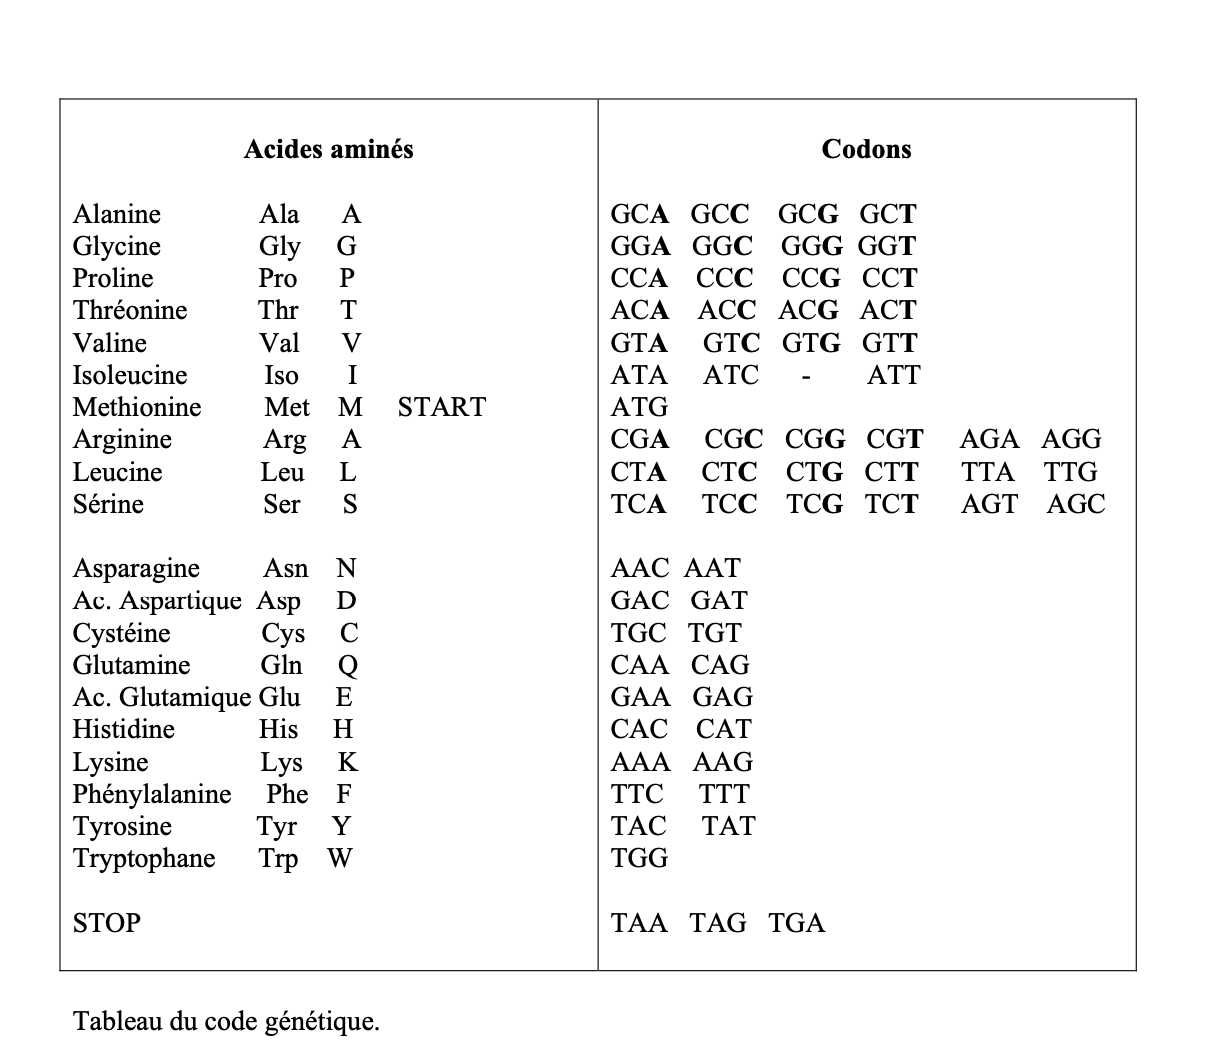
\includegraphics[scale=0.6]{code}
\end{figure}


\begin{correction}

\end{correction}